% Homework template for Algorithm Analysis and Design
% UPDATE: September 20, 2019 by Xu Rongchen
\documentclass[a4paper]{article}
\usepackage{ctex}
\ctexset{
proofname = \heiti{证明} %% set proof name
}
\usepackage{amsmath, amssymb, amsthm}
% amsmath: equation*, amssymb: mathbb, amsthm: proof
\usepackage{moreenum}
\usepackage{mathtools}
\usepackage{url}
\usepackage{bm}
\usepackage{enumitem}
\usepackage{graphicx}
\usepackage{subcaption}
\usepackage{booktabs} % toprule
\usepackage[mathcal]{eucal}

\usepackage{iidef} % set homework count
\usepackage{longtable}

% \usepackage[noend]{algpseudocode}
\usepackage{clrscode3e}

\thecoursename{算法分析与设计实验报告}
\theterm{2019年秋季学期}
\hwname{Fibonacci数求解}
\slname{\heiti{解}}
\begin{document}
\courseheader
\theusername{徐荣琛}
\thestuno{2019214518}
\theinstitute{软件学院}

\info

\begin{enumerate}
  \setlength{\itemsep}{3\parskip}
  %% Homework Start here:
  %% \item to enumerate the problem ID: Format as 'HomeworkID.ProblemID'
  %% \begin{solution} XXXX \end{solution} is to make a solution
  %% \begin{proof} XXXX \end{proof} is to make a proof
  %% Suggest to use \input{path} command
  \textbf{1.实验要求}\\
  比较不同方法求Fibonacci数.\\
  \bigskip

  \textbf{2.实验环境}\\
  实验代码采用C\#语言实现,具体的实验环境如下表所示:\\ \medskip
  \begin{tabular}{c|c}
    \hline\hline
    处理器 & Intel(R) Core(TM) i7-8850H CPU @ 2.60GHz \\ \hline
    内存 & 16GB\\ \hline
    操作系统& Mac OS X 10.14.6\\ \hline
    编译环境& .Net Core 3.0.100\\
    \hline\hline
  \end{tabular}\\
  \bigskip

  \textbf{3.实验内容}\\
  \textbf{3.1 复杂度为$\Theta(\lg n)$的Fibonacci数求解算法实现}\\
  \medskip
  算法实现的具体思路:\\
  Fibonacci数求解的问题转化为求解如下矩阵幂的问题:
  \begin{align*}
    \begin{bmatrix} 
      F_{n+1} & F_n \\
      F_n & F_{n-1}
    \end{bmatrix}
    ={
    \begin{bmatrix} 
      1 & 1 \\
      1 & 0
    \end{bmatrix}
    }^n
  \end{align*}
  (1)实现一个2x2的矩阵类,并根据矩阵运算规则重载加法、乘法运算(为了保证可以处理较大的Fibonacci数,矩阵内的元素采用大数);\\
  (2)重载矩阵的幂运算:若$n==1$直接返回原矩阵,否则:
  \begin{align*}
    M^n=\left\{
    \begin{aligned}
      &M^{\frac{n}{2}} \cdot M^{\frac{n}{2}} \cdot M &(n \% 2 == 1)\\
      &M^{\frac{n}{2}} \cdot M^{\frac{n}{2}} &(n \% 2 == 0)
    \end{aligned}
    \right.
  \end{align*}

  \medskip
  \textbf{3.2 $\Theta(\lg n)$和$\Theta(n)$算法在不同规模数据下的对比实验}\\
  \medskip
  3.2.1 实验概要:\\
  对于两种算法,分别计算3次第1、5、1E1、5E1、1E2、5E2、1E3、5E3、1E4、5E4、
  1E5、5E5、1E6、5E6、1E7、5E7个Fibonacci数,设置每组的超时时间为60秒。
  实验程序编译时设定为Release。\\
  \medskip
  3.2.2 实验结果:\\
  实验结果如下表所示:\\ \medskip
  \resizebox{\linewidth}{!}{ 
  \begin{tabular}{c||ccc|c||ccc|c}
    \hline\hline
    \#& $E1$& $E2$& $E3$& $EA$& $N1$& $N2$& $N3$& $NA$\\ \hline
    1  &0.00060 &0.00061 &0.00059 &0.00060 &0.00166 &0.00138 &0.00081 &0.00128 \\
    5  &0.00077 &0.00049 &0.00054 &0.00060 &0.00016 &0.00008 &0.00008 &0.00011 \\
    1E1&0.00019 &0.00016 &0.00012 &0.00016 &0.00009 &0.00009 &0.00005 &0.00007 \\
    5E1&0.00024 &0.00019 &0.00015 &0.00020 &0.00020 &0.00011 &0.00029 &0.00020 \\
    1E2&0.00013 &0.00014 &0.00014 &0.00014 &0.00037 &0.00020 &0.00011 &0.00023 \\
    5E2&0.00024 &0.00009 &0.00014 &0.00015 &0.00024 &0.00024 &0.00021 &0.00023 \\
    1E3&0.00052 &0.00017 &0.00018 &0.00029 &0.00048 &0.00038 &0.00041 &0.00042 \\
    5E3&0.00111 &0.00071 &0.00076 &0.00086 &0.00325 &0.00322 &0.00293 &0.00314 \\
    1E4&0.00048 &0.00040 &0.00055 &0.00048 &0.00634 &0.00611 &0.00611 &0.00619 \\
    5E4&0.00253 &0.00261 &0.00136 &0.00217 &0.06765 &0.05837 &0.05592 &0.06065 \\
    1E5&0.00608 &0.00627 &0.00628 &0.00621 &0.16915 &0.15830 &0.15746 &0.16163 \\
    5E5&0.06613 &0.06401 &0.06227 &0.06414 &3.08121 &3.35667 &3.51734 &3.31841 \\
    1E6&0.15356 &0.15136 &0.15227 &0.15240 &12.72376&13.13648&14.00214&13.28746\\
    5E6&1.68542 &1.77099 &1.73009 &1.72883 &Timeout&Timeout&Timeout&Timeout\\
    1E7&6.72721 &6.81682 &6.86573 &6.80325 &Timeout&Timeout&Timeout&Timeout\\
    5E7&Timeout&Timeout&Timeout&Timeout&Timeout&Timeout&Timeout&Timeout\\
    \hline\hline
  \end{tabular}
  }\\
  \medskip
  表中,$E1,E2,E3,N1,N2,N3$分别表示高效算法(Efficient)和直接计算(Naive)三次实验的结果,$EA,NA$是三次实验的均值。
  时间单位为秒。\\
  \medskip
  3.2.3 实验分析:\\
  以数据规模为横坐标,算法平均耗时为纵坐标(为方便低数量级的展示,故这里采用对数坐标),绘制出如下的
  耗时曲线比较图:
  \begin{center}
    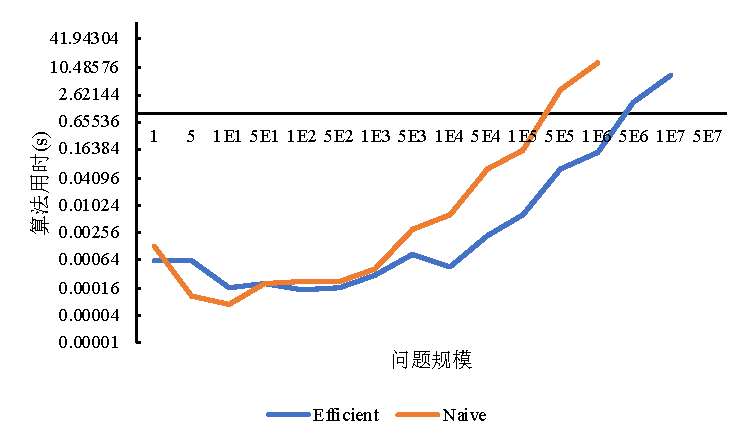
\includegraphics[scale=0.8]{Pictures/Chart.pdf}
  \end{center}
  从图中可发现,总体而言,随着问题规模的增大,算法耗时相应增加。
  当数据规模较小时($10^4$数量级以下),算法耗时有一定的波动。当数据规模超过$10^4$数量级后,
  复杂度为$O(\lg n)$的算法表现出了明显的计算优势。特别的,只有$O(\lg n)$的算法在60秒超时上限内解决了5E6和1E7两个问题。\\
  然而,$O(\lg n)$的算法却不能在限时内解决5E7及更高规模的问题,这直观上与算法的复杂度不符合,分析其原因是当$n$变大时,
  问题中需要计算的大数长度也相应指数级增大,此时算法的复杂度还需要考虑到大数乘法的时间消耗,这也是限制解决问题的规模的主要原因。\\
\end{enumerate}
\end{document}